\documentclass[12pt,a4paper,twoside,openright,titlepage,final]{article}
\usepackage{fontspec}
\usepackage{amsmath}
\usepackage{amsfonts}
\usepackage{amssymb}
\usepackage{makeidx}
\usepackage{graphicx}
\usepackage[hidelinks,unicode=true]{hyperref}
\usepackage[spanish,es-nodecimaldot,es-lcroman,es-tabla,es-noshorthands]{babel}
\usepackage[left=3cm,right=2cm, bottom=4cm]{geometry}
\usepackage{natbib}
\usepackage{microtype}
\usepackage{ifdraft}
\usepackage{verbatim}
\usepackage[obeyDraft]{todonotes}
\ifdraft{
	\usepackage{draftwatermark}
	\SetWatermarkText{BORRADOR}
	\SetWatermarkScale{0.7}
	\SetWatermarkColor{red}
}{}
\usepackage{booktabs}
\usepackage{longtable}
\usepackage{calc}
\usepackage{array}
\usepackage{caption}
\usepackage{subfigure}
\usepackage{footnote}
\usepackage{url}
\setsansfont[Ligatures=TeX]{texgyreadventor}
\setmainfont[Ligatures=TeX]{texgyrepagella}
\setmonofont{FreeMono}

\usetikzlibrary{decorations.pathreplacing}

%*******************************************************
%                 NO MODIFICAR
\newcommand*{\FSfont}[1]{%
  \fontencoding{T1}\fontfamily{#1}\selectfont}

\newlength{\tpheight}\setlength{\tpheight}{0.9\textheight}
\newlength{\txtheight}\setlength{\txtheight}{0.9\tpheight}
\newlength{\tpwidth}\setlength{\tpwidth}{0.9\textwidth}
\newlength{\txtwidth}\setlength{\txtwidth}{0.9\tpwidth}
\newlength{\drop}
%*******************************************************

% Crea una portada con los siguientes parámetros
%
% #1 : Título 
% #2 : Subtítulo
% #3 : Subsubtítulo
% #4 : Autor(es)
% #5 : Lugar
%

\newcommand*{\portada}[5]{
\begin{titlepage}
\begingroup
\vspace*{1cm}
\drop = 0.2\txtheight
\centering
\vfill
{\Huge \scshape #1}\\[\baselineskip]
{\Large \textbf{#2}}\\[\baselineskip]
{\Large \scshape #3}\\[\baselineskip]
\vspace*{0.3cm}
{\large \textit{#4}}\\[0.5\drop]

\includegraphics[scale=0.35]{./imagenes/logoURJC.jpg}
\vspace*{1.5cm}

{\large \scshape #5, \today} \par
\begin{center}
\end{center}
\vfill\null
\endgroup
\end{titlepage}
}
 %*****************************************************
 


\author{José Ignacio Escribano}

\title{}

\setlength{\parindent}{0pt}

\begin{document}

\pagenumbering{alph}
\setcounter{page}{1}

\portada{Ejemplo Práctico}{Calidad Seis Sigma}{Proceso de producción de helicópteros}{José Ignacio Escribano}{Móstoles}

\listoffigures
\thispagestyle{empty}
\newpage

\listoftables
\thispagestyle{empty}
\newpage

\tableofcontents
\thispagestyle{empty}
\newpage


\pagenumbering{arabic}
\setcounter{page}{1}

\section{Definición}

La empresa Parasafe S.A. se dedica al diseño, producción y venta de helicópteros de papel.\\

Estos helicópteros se utilizan para realizar estudios de aerodinámica en diseño de túneles de viento, separadores ciclónicos y sistemas de ventilación especiales.\\

El proceso de fabricación de estos helicópteros consta de cuatro etapas básicas: el aprovisionamiento de materia prima, el montaje, la prueba de vuelo y el etiquetado final previo al envío al cliente.\\

El montaje consta de dos subprocesos: el corte del papel y el pegado del mismo. El corte consiste en separar el borde del patrón y realizar los cortes señalados; el pegado consiste en unir los bordes del cuerpo con cinta adhesiva corriente. El proceso se hace de forma manual.\\

La prueba de vuelo consiste en lanzar cada helicóptero, en posición vertical, desde una altura de 2 metros, y midiendo el tiempo que tarda en caer al suelo. Se considera que el helicóptero pasa la prueba si el tiempo de vuelo es mayor o igual a 1 segundo. La prueba se realiza con un cronógrafo manual, capaz de medir 1/100 segundos.\\

El equipo de producción de Parasafe S.A. consta de 10 personas, que trabajan un único turno de 8 horas/día. El reparto de empleados entre las diferentes tareas es el siguiente:

\begin{itemize}
	\item Etapa de inspección: 1 personas más medio turno de otra
	\item Etapa de corte: 2 personas más medio turno de otra
	\item Etapa de pegado: 1 persona más medio turno de otra
	\item Etapa de la prueba de vuelo: 3 personas
	\item Etapa de etiquetado: 1 persona más medio turno de otra
\end{itemize}

El tiempo que se emplea en la fabricación de un helicóptero se desglosa a continuación:

\begin{itemize}
	\item Etapa de inspección: 35 segundos/unidad
	\item Etapa de corte: 55 segundos/unidad
	\item Etapa de pegado: 35 segundos/unidad
	\item Etapa de la prueba de vuelo: 55 segundos/unidad
	\item Etapa de etiquetado: 35 segundos/unidad
\end{itemize}

Los costes de producción se describen a continuación:

\begin{enumerate}
	\item Costes fijos
	\begin{itemize}
		\item Salario de los empleados
		\begin{itemize}
			\item 1200 €/mes por operario
			\item 1900 €/mes por técnico
		\end{itemize}
		\item Alquiler y gastos de mantenimiento: 4000 €/mes 
	\end{itemize}
	
	\item Coste del papel (tamaño DIN A4)
	\begin{itemize}
		\item Suministrador A (buena calidad): 0.8 €/hoja
		\item Suministrador B (mala calidad): 0.6 €/hoja
	\end{itemize}
	
	\item Coste de inspección: 0.55 €/unidad
	\item Coste del corte: 1.5 €/unidad
	\item Coste del pegado: 0.45 €/unidad
	\item Coste de la prueba de vuelo: 1.5 €/unidad
	\item Coste del etiquetado: 0.55 €/unidad
\end{enumerate}

El precio de venta actual es de 6 €/unidad.\\

Teniendo en cuenta los tiempos diarios dedicados a cada tarea (sumando a todos los empleados) y el tiempo de realización de cada tarea en cada unidad se tiene que las unidades que se pueden realizar en cada tarea son las siguientes:

\begin{table}[htbp!]
	\centering
	\caption{Número de unidades diarias por tareas}
	\label{tbl:tiempos}
	\begin{tabular}{@{}cccc@{}}
		\toprule
		Tarea        & \begin{tabular}[c]{@{}c@{}}Tiempo diario\\ (en horas)\end{tabular} & \begin{tabular}[c]{@{}c@{}}Tiempo en realizar tarea\\ por unidad (en segundos)\end{tabular} & \begin{tabular}[c]{@{}c@{}}Número de \\ unidades diarias\end{tabular} \\ \midrule
		Inspección   & 12                                                                 & 35                                                                                          & 1\,234                                                                  \\
		Corte        & 20                                                                 & 55                                                                                          & 1\,309                                                                  \\
		Pegado       & 12                                                                 & 35                                                                                          & 1\,234                                                                  \\
		Prueba vuelo & 24                                                                 & 55                                                                                          & 1\,570                                                                  \\
		Etiquetado   & 12                                                                 & 35                                                                                          & 1\,234                                                                  \\ \bottomrule
	\end{tabular}
\end{table} 

A la vista de la Tabla~\ref{tbl:tiempos} tenemos una producción de 1\,234 unidades diarias, que al mes son 37\,028 unidades.\\

Estas 37\,028 suponen unos ingresos de 222\,168 € mensuales.\\

Los costes mensuales asociados son de 220\,400 €.\\

Por tanto, el beneficio mensual es de 1\,768.2 €.\\

Los objetivos generales del proyecto son los siguientes:

\begin{itemize}
	\item El tiempo de vuelo debe ser mayor de 1 segundo. Sólo 1 de cada 2000 helicópteros podrá no cumplir este requisito de calidad.
	\item El coste de producción debe ser mínimo
\end{itemize} 



\section{Medida}

En primer lugar, representamos el diagrama del proceso actual. Comenzamos con el diagrama de alto nivel para finalizar con el diagrama completo.\\

Para representar el diagrama del proceso de alto nivel, debemos identificar las entradas (inputs) y salidas (outputs) del proceso. De las primeras identificamos a los empleados, la materia prima (el papel en el que vienen los helicópteros) y las herramientas. De las segundas identificamos solamente al helicóptero. La Figura~\ref{fig:diagrama_proceso_actual_altoç_nivel} el diagrama de alto nivel del proceso actual.\\

\begin{figure}[htbp!]
	\centering
	\begin{tikzpicture}
	\draw (0,0) node[text width=3cm,align=center, thick, draw=black] (entradas)
	{
		Empleados \\
		Papel \\
		Herramientas
	};
	
	\draw (5,0) node[text width=3cm,align=center, thick, draw=black] (proceso)
	{
		\textbf{PROCESO}    
	};
	
	\draw (10,0) node[text width=3cm,align=center, thick, draw=black] (salidas)
	{
		Helicóptero
	};
	
	\draw [->] (entradas) -- (proceso);
	\draw [->] (proceso) -- (salidas);
	
	\draw (0,1) node[text width=3cm,align=center, thick] (proceso)
	{
		\textbf{ENTRADAS}    
	};
	
	\draw (10,1) node[text width=3cm,align=center, thick] (proceso)
	{
		\textbf{SALIDAS}    
	};
	\end{tikzpicture}
	\caption{Diagrama del proceso actual de alto nivel}
	\label{fig:diagrama_proceso_actual_altoç_nivel}
\end{figure} 

Para representar el diagrama del proceso actual, debemos identificar las fases de las que consta el proceso. Éstas son: aprovisionamiento de materia prima, montaje, prueba de vuelo y etiquetado. 

En la fase de aprovisionamiento tenemos como entrada el papel que nos proporcionan, donde un empleado revisa cada hoja midiendo el ancho del patrón y descarta los que no cumplan el criterio (12 $\pm$ 0.1 cm).\\

En la fase de montaje, tenemos como entrada el papel inspeccionado de la fase anterior donde un empleado corta y pega el helicóptero, que es nuestra salida de esta fase. Dentro de esta fase, tenemos dos subprocesos: el corte y el pegado. En el primero, un empleado separa el borde del patrón y realiza los cortes; y el segundo, donde el empleado une los bordes con cinta adhesiva.\\

En la fase de prueba de vuelo, tenemos como entrada nuestro helicóptero ya construido. En esta fase, un empleado mide el tiempo de vuelo del helicóptero desde una altura de dos metros de alto, atendiendo a los siguientes parámetros: largo del ala, largo del cuerpo, ancho del cuerpo, si lleva o no lleva clip, si lleva cinta o si lleva cinta en el cuerpo. Con el tiempo de vuelo, se desechan aquellos que no cumplen el tiempo de vuelo impuesto por el cliente (> 1 segundo).\\

En la última fase, la de etiquetado, un empleado etiqueta los helicópteros (nuestra entrada en esta fase) y descarta los que no cumplen el tiempo de vuelo especificado por el cliente.\\

El diagrama completo del proceso actual se puede ver en la Figura~\ref{fig:diagrama_proceso_actual}\\  

\begin{figure}[htbp!]
	\centering
	\begin{tikzpicture}
	
	% Entradas
	\draw (0,0) node[text depth=2cm,text width=5cm,align=center, thick, draw=black] (entradas)
	{
		\textbf{ENTRADAS}
	};
	
	\node[text width=5cm, align=center] at (entradas.center){Empleados \\ Papel \\ Herramientas};
	
	
	% Aprovisionamiento 
	\draw (0,-3) node[text depth=1cm,text width=5cm,align=center, thick, draw=black] (aprovisionamiento)
	{
		\textbf{APROVISIONAMIENTO}
	};
	
	\node[text width=5cm, align=center] at (aprovisionamiento.center){Papel};
	
	
	% Montaje 
	\draw (0,-6) node[text depth=1.5cm,text width=5cm,align=center, thick, draw=black] (montaje)
	{
		\textbf{MONTAJE}
	};
	
	\node[text width=5cm, align=center] at (montaje.center){Papel \\ inspeccionado};
	
	% Prueba de vuelo 
	\draw (0,-9) node[text depth=2cm,text width=5cm,align=center, thick, draw=black] (prueba)
	{
		\textbf{PRUEBA DE VUELO}
	};
	
	\node[text width=5cm, align=center] at (prueba.center){Helicóptero};
	
	% Etiquetado 
	\draw (0,-12) node[text depth=1cm,text width=5cm,align=center, thick, draw=black] (etiquetado)
	{
		\textbf{ETIQUETADO}
	};
	
	\node[text width=5cm, align=center] at (etiquetado.center){Helicóptero}; 
	
	% Salidas 
	\draw (0,-15) node[text depth=1cm,text width=5cm,align=center, thick, draw=black] (salidas)
	{
		\textbf{SALIDAS}
	};
	
	\node[text width=5cm, align=center] at (salidas.center){Helicóptero};
	
	
	
	% Flechas
	
	\draw [->, thick] (entradas) -- (aprovisionamiento); 
	\draw [->, thick] (aprovisionamiento) -- (montaje);       
	\draw [->, thick] (montaje) -- (prueba);
	\draw [->, thick] (prueba) -- (etiquetado);
	\draw [->, thick] (etiquetado) -- (salidas);                     
	
	
	% Entradas y salidas
	
	\draw (-5,-3) node[text depth=1cm,text width=4cm,align=right, thick]
	{
		empleado \textbf{C} \\
		medir patrón \textbf{P} \\
		descartar \textbf{P}
	};
	
	\draw (-5,-6) node[text depth=1cm,text width=4cm,align=right, thick]
	{
		empleado \textbf{C} \\
		cortar \textbf{P} \\
		pegar \textbf{P}
	};
	
	\draw (-5,-8.5) node[text depth=2.5cm,text width=4cm,align=right, thick]
	{
		empleado \textbf{C} \\
		medir tiempo \textbf{P} \\
		descartar \textbf{P} \\
		largo ala \textbf{C} \\
		ancho cuerpo \textbf{C} \\
		clip, cinta \textbf{C} \\
		cinta cuerpo \textbf{C} \\
		velocidad viento \textbf{NC}
	};
	
	\draw (-5,-12) node[text depth=1cm,text width=4cm,align=right, thick]
	{
		empleado \textbf{C} \\
		etiquetar \textbf{P} \\
		descartar \textbf{P}
	};
	
	% Corte y pegado
	\draw (5,-4) node[text depth=1cm,text width=3cm,align=center, thick, draw=black] (corte)
	{
		\textbf{CORTE}
	};
	\node[text width=3cm, align=center] at (corte.center){Helicóptero};
	
	
	\draw (5,-8) node[text depth=1cm,text width=3cm,align=center, thick, draw=black] (pegado)
	{
		\textbf{PEGADO}
	};
	
	\node[text width=3cm, align=center] at (pegado.center){Helicóptero};
	
	
	\draw [->, thick] (corte) -- (pegado);
	
	
	% Llave
	\draw [decorate,decoration={brace,amplitude=10pt},xshift=-40pt,yshift=0pt, thick]
	(4.5,-9) -- (4.5,-3) node [black,midway,xshift=-0.6cm] 
	{\footnotesize $ $};
	
	
	\draw (9,-4) node[text depth=1cm,text width=4cm,align=left, thick]
	{
		\textbf{C} empleado  \\
		\textbf{P} separar  \\
		\textbf{P} cortar 
	};
	
	
	\draw (9,-8) node[text depth=1cm,text width=4cm,align=left, thick]
	{
		\textbf{C} empleado  \\
		\textbf{P} unir
	};
	
	
	\end{tikzpicture}
	\caption{Diagrama del proceso actual}
	\label{fig:diagrama_proceso_actual}
\end{figure} 

Una vez que hemos definido el diagrama de proceso actual, estamos en disposición de analizar el sistema de medida actual con la técnica R\&R (Repetibilidad y Reproducibilidad).\\

Para ello, definimos tres prototipos de helicópteros (Tabla~\ref{tbl:prototipos}) con distintas características de diseño y medimos el tiempo de vuelo dos veces por cada uno de los tres operarios (A, B y C).\\

\begin{table}[htbp!]
	\centering
	\caption{Tres prototipos de helicópteros}
	\label{tbl:prototipos}
	\begin{tabular}{@{}cccc@{}}
		\cmidrule(l){2-4}
		& Prototipo Nº1 & Prototipo Nº2 & Prototipo Nº3 \\ \midrule
		Clip         & Sí            & Sí            & No            \\
		Celo ala     & Sí            & Sí            & Sí            \\
		Celo cuerpo  & Sí            & Sí            & Sí            \\
		Largo ala    & 8             & 6.5           & 9.5           \\
		Largo cuerpo & 8             & 8             & 6.5           \\
		Ancho cuerpo & 5             & 5             & 5             \\ \bottomrule
	\end{tabular}
\end{table}

Por lo que debemos realizar 18 mediciones del tiempo de vuelo. Estos tiempos de vuelo se pueden ver en la Tabla~\ref{tbl:tiempos_operario}.

\begin{center}
	\begin{longtable}{ccc}
		\caption{Tiempos de vuelo por prototipo y tiempo de vuelo}\\
		\label{tbl:tiempos_operario} \\
		\hline
		Prototipo & Operario & Tiempo \\
		\hline
		\endfirsthead
		\multicolumn{3}{c}%
		{\tablename\ \thetable\ -- \textit{Continúa de la página anterior}} \\
		\hline
		Prototipo & Operario & Tiempo \\
		\hline
		\endhead
		\hline \multicolumn{3}{r}{\textit{Continúa en la página siguiente}} \\
		\endfoot
		\hline
		\endlastfoot
		3         & B        & 2.271  \\
		1         & B        & 1.391  \\
		3         & B        & 2.365  \\
		2         & C        & 1.025  \\
		1         & A        & 1.392  \\
		2         & B        & 0.854  \\
		1         & A        & 1.47   \\
		3         & A        & 2.467  \\
		3         & C        & 2.026  \\
		2         & B        & 0.799  \\
		1         & C        & 1.409  \\
		2         & A        & 1.152  \\
		3         & A        & 2.335  \\
		1         & C        & 1.267  \\
		1         & B        & 1.041  \\
		2         & A        & 1.318  \\
		2         & C        & 0.679  \\
		3         & C        & 2.133  \\
	\end{longtable}
\end{center}
		
Con esta información ya estamos en disposición de analizar el sistema de medida. Para ello, introducimos los datos en Minitab y ejecutamos el comando para analizar el sistema de medida.\\

La salida de Minitab es la siguiente:

\begin{verbatim}
Tabla ANOVA de dos factores con interacción 

Fuente                      GL       SC       MC        F      P
Prototipo                 2  5,36825  2,68412  94,7562  0,000
Operario                  2  0,25410  0,12705   4,4851  0,095
Prototipo * Operario   4  0,11331  0,02833   1,5141  0,277
Repetibilidad                9  0,16838  0,01871
Total                       17  5,90403


α para eliminar el término de interacción = 0,05


Tabla ANOVA dos factores sin interacción 

Fuente         GL       SC       MC        F      P
Prototipo    2  5,36825  2,68412  123,875  0,000
Operario     2  0,25410  0,12705    5,863  0,015
Repetibilidad  13  0,28168  0,02167
Total          17  5,90403


R&R del sistema de medición 

                              %Contribución
Fuente               CompVar   (de CompVar)
Gage R&R total      0,039231           8,12
  Repetibilidad     0,021668           4,49
  Reproducibilidad  0,017563           3,64
    Operario        0,017563           3,64
Parte a parte       0,443743          91,88
Variación total     0,482974         100,00


%Var.
Desv.Est.  Var. estudio  estudio
Fuente                   (DE)      (6 × DE)    (%VE)
Gage R&R total       0,198069       1,18841    28,50
  Repetibilidad      0,147200       0,88320    21,18
  Reproducibilidad   0,132527       0,79516    19,07
    Operario         0,132527       0,79516    19,07
Parte a parte        0,666140       3,99684    95,85
Variación total      0,694963       4,16978   100,00


Número de categorías distintas = 4
\end{verbatim}

De la salida se desprende que el sistema de medición es bastante bueno, ya que el R\&R total es del 8.12\%, inferior al 10\%. Además, el número de categorías distintas es 4.\\

Además, vemos que la repetibilidad es del 4.49\% y la reproducibilidad es del 3.64\% (sólo aporta Operario y no hay interacción entre Prototipo y Operario). La aportación Parte a Parte es del 91.88\%.\\

En la Figura~\ref{fig:R&RdelsistemademediciónparaTiempo} se puede observar el informe del sistema de medición de forma más gráfica. Se puede observar en la gráfica Componentes de variación lo comentado anteriormente: el R\&R total del sistema es muy bajo, por debajo del 10\% (concretamente del 8.12\%). En gráfica R por Operario se observa que que todos los puntos se encuentran dentro de los límites de control. En la gráfica Xbarra por Operario, se observa que la mayoría de puntos se encuentran fuera de control. En la gráfica Tiempo por Prototipo, vemos que el prototipo 3 destaca notablemente con respecto a los otros 2 en el tiempo de vuelo. Este prototipo parece que es el mayor tiempo de vuelo ofrece de los tres prototipos. En la gráfica de Tiempo por Operario, parece que el operario influye poco o muy poco en el tiempo total de vuelo de nuestro helicóptero. Por último, en la gráfica de Interacción Prototipo*Operario, parece que hay poca interacción, ya que hay poca diferencia en el tiempo de vuelo según el prototipo y el  operario.\\

\begin{figure}[htbp!]
	\centering
	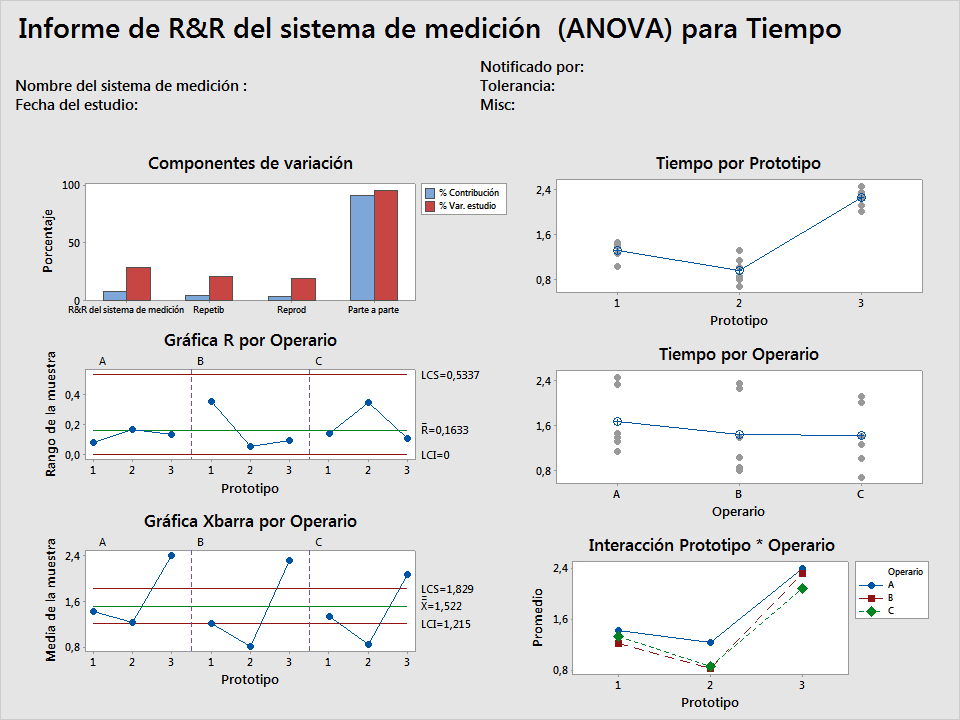
\includegraphics[width=0.7\linewidth]{imagenes/RR_del_sistema_de_medicion_para_Tiempo}
	\caption{R\&R del sistema de medición}
	\label{fig:R&RdelsistemademediciónparaTiempo}
\end{figure}

Ahora, procedemos a realizar el análisis de capacidad del proceso actual. Para ello, tomamos 20 medidas del tiempo de vuelo para un mismo prototipo. En nuestro caso, el prototipo 2. Los tiempos de vuelo recogidos se pueden ver la Tabla~\ref{tbl:tiempos_capacidad}.\\

\begin{center}
	\begin{longtable}{ccc}
		\caption{Tiempos de vuelo del prototipo 2 para calcular la capacidad del proceso}\\
		\label{tbl:tiempos_capacidad} \\
		\hline
		Tiempo \\
		\hline
		\endfirsthead
		\multicolumn{1}{c}%
		{\tablename\ \thetable\ -- \textit{Continúa de la página anterior}} \\
		\hline
		Tiempo \\
		\hline
		\endhead
		\hline \multicolumn{1}{r}{\textit{Continúa en la página siguiente}} \\
		\endfoot
		\hline
		\endlastfoot
		1.150  \\
		1.574  \\
		1.210  \\
		1.471  \\
		1.234  \\
		1.294  \\
		1.471  \\
		1.057  \\
		1.138  \\
		1.110  \\
		0.971  \\
		1.067  \\
		1.072  \\
		1.199  \\
		1.177  \\
		1.305  \\
		1.287  \\
		1.188  \\
		0.964  \\
		1.134  \\
	\end{longtable}
\end{center}

Antes de calcular la capacidad del proceso, comprobamos si los datos están distribuidos de acuerdo a una distribución normal. Para ello, aplicamos el test de Anderson-Darling en Minitab. Los resultados de este test se pueden ver en la Figura~\ref{fig:normalidad_capacidad}.\\

\begin{figure}[htbp!]
	\centering
	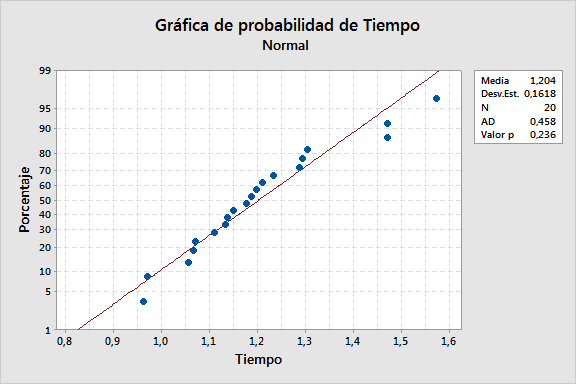
\includegraphics[width=0.7\linewidth]{imagenes/Grafica_de_normalidad_de_Tiempo_(analisis_de_capacidad)}
	\caption{Resultado del test de Anderson-Darling}
	\label{fig:normalidad_capacidad}
\end{figure}

El test arroja un p-valor de 0.236, mayor que 0.05. Por lo que no tenemos evidencia para rechazar la hipótesis de que los datos siguen una distribución normal.\\

Ya estamos en disposición de calcular la capacidad del proceso actual. El resultado del análisis de capacidad se puede ver en la Figura~\ref{fig:capacidad_actual}.\\ 

\begin{figure}[htbp!]
	\centering
	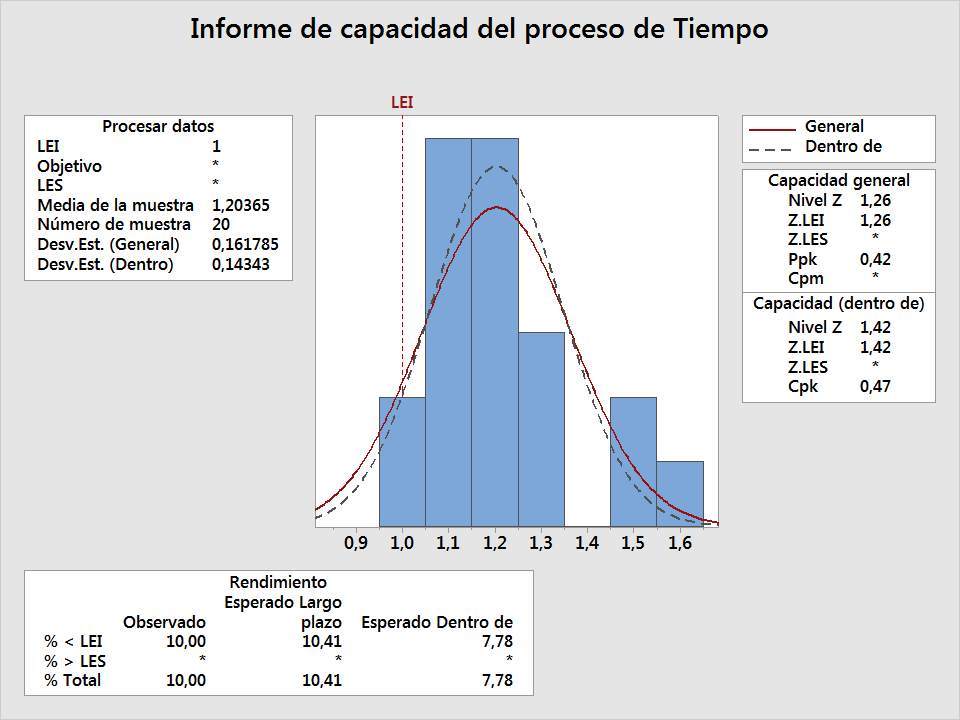
\includegraphics[width=0.7\linewidth]{imagenes/Informe_de_capacidad_del_proceso_de_Tiempo}
	\caption{Análisis de capacidad del proceso actual}
	\label{fig:capacidad_actual}
\end{figure}

Vemos que nuestro proceso tiene 1.26 sigmas, por lo que tenemos un gran margen de mejora en el proceso actual. Si siguiéramos con este proceso a largo plazo, nuestro proceso mejoraría hasta las 1.42 sigmas, insuficiente para los objetivos que marca el cliente.\\

Antes de analizar las causas que influyen en el tiempo de vuelo de nuestro helicóptero, debemos determinar las causas que pueden afectar al tiempo de vuelo. Para ello, aplicamos la regla de las 6 M's (mediciones, material, personal, medio ambiente, métodos y máquinas)\\

En el grupo de las mediciones identificamos como causas el largo de ala, el ancho del cuerpo y largo del cuerpo. En material identificamos la calidad y el peso. En personal, la experiencia, la motivación y la formación. En el medio ambiente, la velocidad del viento. En métodos la calidad del corte, del doblado y del pegado y la prueba de vuelo. Por último, en máquinas identificamos la edad y el mantenimiento. Todo esto se puede ver de forma gráfica en el diagrama de causas y efectos o diagrama de Ishikawa (Figura~\ref{fig:causa_efecto}).\\


\begin{figure}[htbp!]
	\centering
	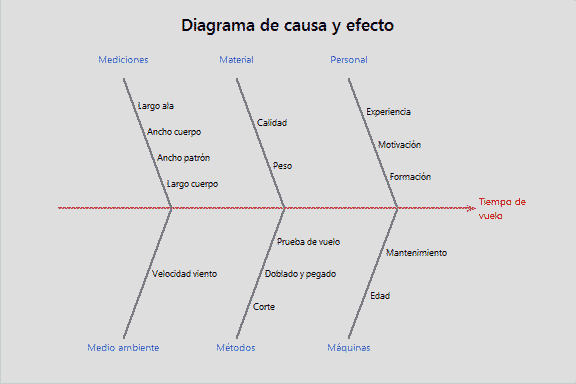
\includegraphics[width=0.7\linewidth]{imagenes/Diagrama_de_causa_y_efecto}
	\caption{Diagrama de causas y efectos para el tiempo de vuelo}
	\label{fig:causa_efecto}
\end{figure}


\section{Análisis gráfico}

\subsection{Análisis numérico}

\section{Mejora}

\subsection{Optimización del diseño y del proceso de fabricación}

\section{Control}

\section{Conclusiones}



\end{document}